%\section{Decisions}
%\section{Implementation}
%\section{Outcomes}
%Main result(s) and their scientific evidence
%\section{Summary}

\section{Autorização de pedidos à \acrshort{api}}

Quanto à forma como os pedidos serão feitos à \acrshort{api} poderão ser feitos de duas formas, através da \textit{header} \acrshort{http} \textit{Authorization} ou através da \textit{query string} do pedido em um dos seguintes campos:
\begin{itemize}[leftmargin=3cm]
    \item[\textbf{\texttt{token}}] caso seja o \texttt{token} de um utilizador:\newline
        \verb|http://example.com/path/page?token=<token>|
    \item[\textbf{\texttt{apikey}}] caso seja uma Chave \acrshort{api}:\newline
        \verb|http://example.com/path/page?apikey=<Chave API>|
\end{itemize}

Na \textit{header} \textit{Authorization} irá ser usado o esquema de autenticação \textit{Bearer}\footnote{Mais informação em \url{https://tools.ietf.org/html/rfc6750}} com umas pequenas alterações. Portanto o conteúdo da \textit{header} \textit{Authorization}:
\begin{itemize}[leftmargin=2cm]
    \item Caso seja o \texttt{token} de um utilizador é:\newline
        \verb|token <token>|
    \item Caso seja uma Chave \acrshort{api} é:\newline
        \verb|apikey <Chave API>|
\end{itemize}
ao invés do esquema de autenticação predefinido do \textit{Bearer}: \verb|Bearer <token/Chave API>|

Convém referir que a Chave \acrshort{api} é também um \textit{token}. A divisão entre utilizadores e chaves \acrshort{api} permite uma mais fácil gestão dos \textit{tokens} recebidos pela \acrshort{api} bem como usar duas formas diferentes de os gerar/verificar com o possível benefício de melhorar a segurança da \acrshort{api}.

Os \textit{token}s gerados pela \acrshort{api} serão \acrshort{jwt}s. Contudo poderiam ser outro tipo de \textit{tokens} (por exemplo uma \textit{string} aleatória e única) que o processo de envio dos \textit{tokens} para a \acrshort{api} manter-se-ia igual.

Após descrito como poderão ser feitos os pedidos à \acrshort{api}, irá ser apresentado possíveis fluxos de interação entre utilizadores (\textit{browser}, \textit{app}, etc) e o servidor da \acrshort{api}.

O fluxo de autenticação de um utilizador na \acrshort{api} a ser implementado será o seguinte:
\begin{figure}[H]
    \begin{center}
        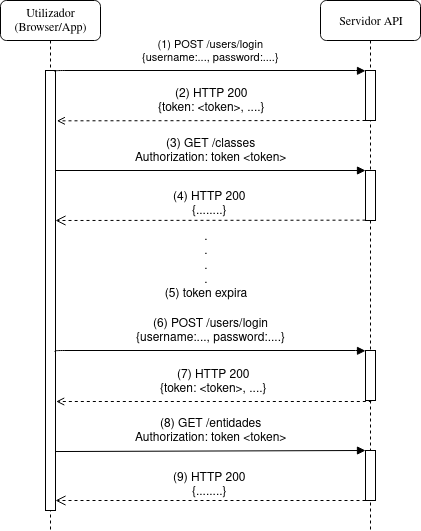
\includegraphics[width=0.5\textwidth]{img/userAuth.png}
    \end{center}
    \caption{Fluxo de autenticação e posteriores pedidos de um utilizador}\label{fig:userAuth}
\end{figure}

\begin{enumerate}
    \item Utilizador autentica-se ao providenciar o seu \textit{email} e a sua \textit{password}
    \item Caso o utilizador se autentique com sucesso é devolvido um \textit{token} que deve ser usado nos restantes pedidos até expirar
    \item Utilizador realiza um pedido para obter as classes, colocando o token na \textit{header} \textit{Authorization}
    \item Caso o \textit{token} enviado seja válido e não tenha expirado são devolvidas as classes
    \item \textit{Token} expirou após o tempo definido
    \item Utilizador realiza uma nova autenticação por forma a obter um novo \textit{token}
    \item Caso o utilizador se autentique com sucesso é devolvido um \textit{token} que deve ser usado nos restantes pedidos até expirar
    \item Utilizador realiza um pedido para obter as entidades, colocando o token na \textit{header} \textit{Authorization}
    \item Caso o \textit{token} enviado seja válido e não tenha expirado são devolvidas as entidades
\end{enumerate}

O fluxo de autenticação e renovação de uma Chave \acrshort{api} na \acrshort{api} a ser implementado será o seguinte:
\begin{figure}[H]
    \begin{center}
        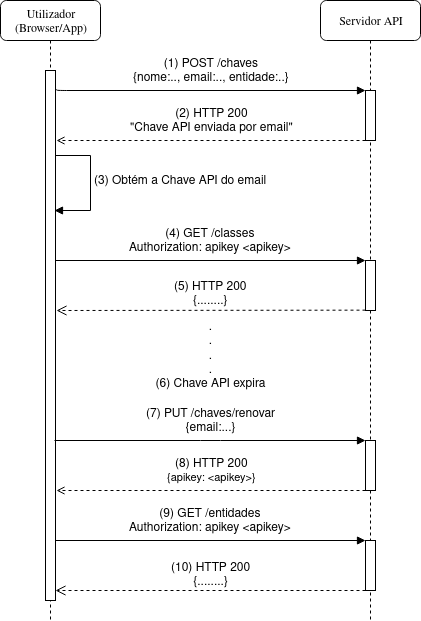
\includegraphics[width=0.5\textwidth]{img/chaveAuth.png}
    \end{center}
    \caption{Fluxo de autenticação e posteriores pedidos de uma chave \acrshort{api}}\label{fig:chaveAuth}
\end{figure}

\begin{enumerate}
    \item Utilizador cria uma chave \acrshort{api} ao providenciar o nome, email e entidade
    \item A Chave \acrshort{api} é enviada para o email fornecido pelo utilizador com o objetivo de ser usada nos próximos pedidos
    \item O utilizador obtém a chave \acrshort{api} do email enviado
    \item Utilizador realiza um pedido para obter as classes, colocando a chave \acrshort{api} na \textit{header} \textit{Authorization}
    \item Caso a Chave \acrshort{api} enviada seja válida e não tenha expirado são devolvidas as classes
    \item Chave \acrshort{api} expirou após o tempo definido
    \item Utilizador renova a Chave \acrshort{api} ao providenciar o email usado para criar a Chave \acrshort{api}
    \item A nova (renovada) Chave \acrshort{api} é devolvida para ser usada nos restantes pedidos
    \item Utilizador realiza um pedido para obter as entidades, colocando a Chave \acrshort{api} na \textit{header} \textit{Authorization}
    \item Caso a Chave \acrshort{api} enviada seja válida e não tenha expirado são devolvidas as entidades
\end{enumerate}

\subsection{Verificação dos \textit{tokens} no servidor \acrshort{api}}

Para proteger as rotas da \acrshort{api} é necessário haver métodos de verificação dos \textit{tokens} com o objetivo de decidir se o utilizador/Chave \acrshort{api} pode aceder a uma determinada rota. De seguida será apresentado o pseudo-código de verificação dos \textit{tokens} tendo em conta que os utilizadores registados conseguem aceder a todas as rotas que as Chaves \acrshort{api} conseguem mas que o inverso não acontece. Ou seja, um utilizador registado até o de nível mais baixo por exemplo, consegue aceder a todas as rotas que as Chaves \acrshort{api} tem acesso e mais algumas nas quais as Chaves \acrshort{api} não têm permissões de acesso.

Por forma a validar se uma Chave \acrshort{api} pode aceder a uma determinada rota pode ser executada a seguinte função em \textit{middleware}:
\begin{lstlisting}[language=pseudocode, caption=Verificação se um pedido com uma determinada Chave \acrshort{api} pode ser efetuado]
function isLoggedInKey(req, res, next)
    key = getJWTfromHeaderOrQueryString('apikey')

    if key then
        keyBD = getKeyFromMongoDB(key)
        if keyBD then
            res = jwt.verify(key, secretForAPIkey)
            if res != expired then
                if keyBD.active == True then
                    return next()
                else
                    return err
            else
                return err
        else
            return err
    else
        return isLoggedInUser(req, res, next)
\end{lstlisting}
É importante destacar a chamada da função \texttt{isLoggedInUser} que é executada no caso de não ser detetado uma Chave \acrshort{api} no pedido (na \textit{header} \textit{Authorization} ou na \textit{query string} \texttt{apikey}) e como tal, com essa chamada, tenta-se perceber se afinal foi passado um \textit{token} de um utilizador já que todos os utilizadores conseguem aceder às rotas que as Chaves \acrshort{api} conseguem como já referido.

No seguimento, para validar se um determinado \textit{token} de um utilizador registado pode aceder a uma determinada rota é executada a seguinte função em \textit{middleware}:
\begin{lstlisting}[language=pseudocode, caption=Verificação se um pedido com um determinado \textit{token} de um utilizador registado pode ser efetuado]
JWTstrategy = passport-jwt.Strategy

passport.use("jwt", new JWTstrategy(
    secretOrKey: secret,
    algorithms: ["HS256"],
    jwtFromRequest: getJWTfromHeaderOrQueryString('token')
, (token, done) => done(null, token)))

function isLoggedInUser(req, res, next)
    passport.authenticate("jwt", { session: false }, function (err, user, info)
        if err then
            return err
        if !user then
            return err
        req.logIn(user, function(err)
            if err then
                return err

            next()
        )
    )(req, res, next)
\end{lstlisting}

Os \textit{tokens} tanto das Chaves \acrshort{api} como de \textit{tokens} de utilizadores registados são obtidos através da utilização de extratores presentes na estratégia \texttt{passport-jwt} do \texttt{passport}. Assim para extrair o \textit{token} da \textit{query string} basta:
\begin{lstlisting}[language=javascript, caption=Extração do \textit{token} da \textit{query string}]
var ExtractJWT = require("passport-jwt").ExtractJwt
token = ExtractJWT.fromUrlQueryParameter("<nome do campo, 'token' ou 'apikey' no caso da CLAV>")
\end{lstlisting}
Já para extrair o \textit{token} da \textit{header} \textit{Authorization} basta:
\begin{lstlisting}[language=javascript, caption=Extração do \textit{token} da \textit{heaer} \textit{Authorization}]
var ExtractJWT = require("passport-jwt").ExtractJwt
token = ExtractJWT.fromAuthHeaderWithScheme("<palavra antes do token, 'Bearer' no caso dum bearer token, 'token' ou 'apikey' no caso da CLAV>")
\end{lstlisting}

Para verificar se o utilizador registado tem um nível suficiente para aceder a uma rota, depois de se verificar que o utilizador está autenticado (\texttt{isLoggedInUser}), deve-se executar também em \textit{middleware} a seguinte função:
\begin{lstlisting}[language=pseudocode, caption=Verificação se um utilizador registado tem permissões suficientes para aceder a uma determinada rota]
function checkLevel(clearance)
    return function(req, res, next)
        havePermissions = False

        if clearance is Array then
            if req.user.level in clearance then
                havePermissions = True
        else
            if req.user.level >= clearance then
                havePermissions = True

        if havePermissions then
            return next()
        else
            return err
\end{lstlisting}
Ou seja, a variável \texttt{clearance} poderá ser uma lista de números ou apenas um número. No primeiro caso verifica-se que o nível do utilizador está presente na lista, em caso afirmativo então o utilizador tem permissões para aceder. Já no segundo caso, o utilizador só terá permissões para aceder se o seu nível foi igual ou superior ao \texttt{clearance}.

Com estas três funções (\texttt{isLoggedInKey}, \texttt{isLoggedInUser} e \texttt{checkLevel}) é possível proceder à proteção da \acrshort{api} da \acrshort{clav} garantindo que utilizadores com diferentes níveis de acesso apenas conseguem aceder ao que lhes é permitido.

\section{Exportação de dados}
Um dos requisitos da \acrshort{api} da \acrshort{clav} é permitir a exportação de Classes, Entidades, Tipologias e Legislações em formato \acrshort{json}, \acrshort{xml} e \acrshort{csv}. Deve também permitir exportar toda a ontologia do projeto nos formatos \acrshort{turtle}, \acrshort{json-ld} e \acrshort{rdf}/\acrshort{xml}.

Para a primeira parte foi necessário desenvolver dois conversores, de \acrshort{json} para \acrshort{xml} e de \acrshort{json} para \acrshort{csv} visto que o \acrshort{json} já é por predefinição devolvido.

\subsection{\acrshort{xml}}
O conversor de \acrshort{json} para \acrshort{xml} criado é representado pelo algoritmo presente no anexo~\ref{exem:convXML}.

Apresenta-se no anexo~\ref{conv:jsonTOxml} uma conversão exemplo.

\subsection{\acrshort{csv}}

Da mesma forma que o \acrshort{xml}, o \acrshort{csv} é convertido sem recurso a uma biblioteca que converta já de si o \acrshort{json} para \acrshort{csv} visto que cada objeto \acrshort{json} a exportar necessita de uma exportação personalizada para \acrshort{csv}. Ao contrário do conversor desenvolvido para \acrshort{xml}, o conversor para \acrshort{csv} não converte qualquer objeto para \acrshort{csv} mas apenas um conjunto restrito de objetos \acrshort{json}.

O algoritmo de conversão de \acrshort{json} para \acrshort{csv} desenvolvido pode ser visualizado no anexo~\ref{exem:convCSV}.

O conjunto de objetos permitidos é lista de classes, de entidades, de tipologias e de legislações e objeto de classe, de entidade, de tipologia e de legislação.

Quanto à conversão em si, possui uma estrutura interna durante a conversão. Esta estrutura é uma lista de listas, em que cada lista representa uma linha do \acrshort{csv}. Cada elemento de uma das listas representará uma célula do \acrshort{csv}. A primeira lista será a primeira linha do \acrshort{csv} e como tal possuirá os títulos. As restantes listas serão as linhas seguintes do \acrshort{csv} em que cada elemento possuirá os valores já transformados em \textit{strings} dos campos dos objetos.

Para além desta estrutura interna existe um dicionário que permite agilizar o algoritmo de conversão. Este dicionário possuirá vários dicionários, um por cada objeto (Classe, Entidade, Tipologia e Legislação) em que cada um destes dicionários irá ter como chaves os campos a converter. Para cada um destes campos existe um tuplo em que na primeira posição está presente o título a colocar no \acrshort{csv} referente a este campo e na segunda posição a função de transformação a executar para o valor do campo. Há a presença de três casos especiais:
\begin{itemize}
    \item Quando o valor do campo é uma lista de objetos e pretendemos apenas um dos campos de cada objeto, o valor do campo deve ser \verb|campo_campoDoObjeto| e deve ser usada a função de transformação \verb|map_value(<campoDoObjeto>)|
    \item Quando o valor do campo é um objeto do qual irá resultar vários títulos, na primeira posição do tuplo deve estar presente uma \textit{string} vazia e a função de transformação deve devolver uma lista com duas posições, na primeira com os títulos e na segunda com os valores transformados dos campos
    \item Quando o valor do campo é uma lista de objetos Classe, Entidade, Tipologia ou Legislação a primeira posição do tuplo deve ser \texttt{null} e a função de transformação deve devolver uma lista de listas sem a primeira linha de títulos
\end{itemize}
No caso da conversão de um objeto e consoante a transformação (ou seja, o título do dicionário) a inserção realizada na lista de listas varia:
\begin{itemize}
    \item \verb|título == null|: concatena-se a lista de listas devolvida pela função de transformação à lista de listas
    \item \verb|título == ""|: concatena-se a lista dos elementos da primeira linha devolvida pela função de transformação com os elementos da primeira linha e realiza-se o mesmo para o caso da segunda linha devolvida, concatena-se a segunda linha com a segunda linha
    \item Nos restantes casos protege-se\footnote{colocar valor entre aspas (\texttt{"})} o título presente no dicionário e adiciona-se à primeira lista; para além disso, o valor transformado devolvido pela função de transformação é adicionado já protegido à segunda lista.
\end{itemize}

No caso da conversão de uma lista de objetos, para cada objeto será feita a conversão já apresentada para um objeto, onde depois é ignorada a linha dos títulos em todos os objetos exceto no primeiro objeto da lista onde é mantido os títulos gerados. Ou seja, na primeira linha estará presente os títulos e nas seguintes linhas, em cada linha estará presente os valores de um objeto.

O último passo seja para uma lista ou para um único objeto é transformar a estrutura interna no \acrshort{csv}. Este papel é desempenhado pela função \texttt{joinLines} em que os elementos de cada lista da lista são juntos de acordo com um separador (neste caso é usado o ponto e vírgula, ``\texttt{;}'') tornando a lista de listas numa lista de \textit{strings}. Por fim, as \textit{strings} desta lista são juntas através da inserção de novas linhas (\texttt{``\textbackslash{}n}'') entre cada \textit{string} gerando o \acrshort{csv} final.

No anexo~\ref{conv:jsonTOcsv} apresenta-se um exemplo de uma conversão, onde o ficheiro \acrshort{json} a converter é o mesmo usado para exemplificar a conversão de \acrshort{xml} presente em~\ref{exem:json}.

\subsection{Exportação da Ontologia}
Por fim quanto à exportação da ontologia, das três é a mais simples visto que o \textit{GraphDB}\footnote{\acrfull{bd} Semântica baseada em grafos compatível com os padrões \acrshort{w3c}. Suporta \acrshort{rdf} e \acrshort{sparql}} possui funcionalidades de exportação dos triplos presentes numa \acrshort{bd} armazenada no \textit{GraphDB}.

Para um fácil uso e compatibilidade com os \textit{standards} da indústria, o \textit{GraphDB} implementou as interfaces da \textit{framework} \textit{RDF4J}, a especificação do protocolo \acrshort{w3c} \acrshort{sparql}\footnote{Ver \url{https://www.w3.org/TR/sparql11-protocol/}} e suporta vários formatos de serialização \acrshort{rdf}\footnote{\label{fnRDF}\textit{TriG}, \textit{BinaryRDF}, \textit{TriX}, \textit{N-Triples}, \textit{N-Quads}, \acrshort{n3}, \acrshort{rdf}/\acrshort{xml}, \acrshort{rdf}/\acrshort{json}, \acrshort{json-ld} e \acrshort{turtle}}.~\cite{graphdbAbout}

O \textit{GraphDB} é um \textit{plugin} \acrshort{sail} para a \textit{framework} \textit{RDF4J} fazendo uso extensivo dos recursos e infraestrutura do \textit{RDF4J} especialmente do modelo \acrshort{rdf}, dos \textit{parsers} \acrshort{rdf} e dos motores de pesquisa.~\cite{graphdbArch}

Assim, o \textit{GraphDB} possui uma \acrshort{rest} \acrshort{api} do servidor RDF4J\footnote{Ver \url{https://rdf4j.org/documentation/rest-api/}} a partir da qual é possível obter todos os triplos de uma \acrshort{bd} através da rota
\begin{verbatim}
<url do GraphDB>/repositories/<id do repositório (BD)>/statements
\end{verbatim}
indicando no cabeçalho \acrshort{http} \textit{Accept} o formato de serialização \acrshort{rdf}\footnoteref{fnRDF} de saída (\textit{\acrshort{mime} type}\footnote{\textit{Standard} que indica a natureza e o formato de um documento, ficheiro ou conjunto de \textit{bytes}. Ver \href{https://tools.ietf.org/html/rfc6838}{RFC 6838}}) dos triplos. Dos vários formatos de serialização \acrshort{rdf} serão apenas suportados (acessíveis) na \acrshort{clav}, como já indicado, o \acrshort{turtle} (\texttt{text/turtle}), o \acrshort{json-ld} (\texttt{application/ld+json}) e o \acrshort{rdf}/\acrshort{xml} (\texttt{application/rdf+xml}).

Apesar da facilidade de exportação da ontologia estes pedidos de exportação originam um grande consumo de recursos de \textit{hardware} por parte do \textit{GraphDB} visto que cada pedido devolve todos os triplos de uma \acrshort{bd} (a atual \acrshort{bd} da \acrshort{clav} possui já cerca de 150 000 triplos explícitos e cerca de 85 000 triplos implícitos) para além da conversão necessária desses triplos para o formato de serialização \acrshort{rdf} de saída. Deve-se então limitar o número de pedidos de exportação realizados ao \textit{GraphDB}. Para tal irá ser usado o seguinte mecanismo de controlo/\textit{cache}:

\begin{itemize}
    \item Os ficheiros exportados são mantidos pela \acrshort{api} da \acrshort{clav}
    \item Mantém-se dois ficheiros por cada serialização \acrshort{rdf}, um com os triplos explícitos e outro com os triplos explícitos e implícitos.
    \item Se o ficheiro pretendido não existe na \acrshort{api} da \acrshort{clav} realiza-se o pedido de exportação ao \textit{GraphDB}
    \item Se o ficheiro pretendido existe na \acrshort{api} da \acrshort{clav} mas não é atualizado há sete dias realiza-se o pedido de exportação ao \textit{GraphDB}
    \item Se o ficheiro pretendido existe na \acrshort{api} da \acrshort{clav} e foi atualizado há menos de sete dias devolve-se ao utilizador o ficheiro guardado na \acrshort{api} da \acrshort{clav}
    \item Mantém-se na \acrshort{api} da \acrshort{clav} apenas o ficheiro mais recente para cada versão de cada serialização \acrshort{rdf}
    \item Cada ficheiro é apenas atualizado (removendo o antigo) quando é feito um pedido por um utilizador desse ficheiro
\end{itemize}

Assim, respeitando todas estas restrições, são mantidas pela \acrshort{api} da \acrshort{clav} no máximo seis ficheiros, dois por cada serialização \acrshort{rdf}. Para além disso estes ficheiros são atualizados no melhor caso de sete em sete dias e no pior caso nunca se o ficheiro nunca for requisitado pelos utilizadores.

\subsection{Exportação na \acrshort{api} de dados}
Nesta secção será explicado de que forma será possível exportar os dados da \acrshort{api}. Para tal definiu-se a \textit{query string} \texttt{fs} (formato de saída) onde é possível indicar claro está o formato de saída. Esta \textit{query string} estará presente nas rotas onde será possível exportar os dados. Para além disso, nestas rotas também se pode indicar o formato de saída através do cabeçalho \texttt{Accept}.

De seguida são apresentadas as rotas onde é possível realizar exportação, os formatos de saída disponíveis para cada rota bem como os valores a usar de forma a obter uma exportação nesse formato:
\begin{table}[H]
    \footnotesize
    \begin{center}
    \begin{tabular}{| m{4cm} | m{9cm}|}
    \hline
    Rota & Formato de saída (valor a usar) \\ \hline
    \texttt{GET /api/classes} & \multirow{8}{9cm}{
        \begin{itemize}
            \setlength\itemsep{0em}
            \item \acrshort{json} (\texttt{json} ou \texttt{application/json})
            \item \acrshort{xml} (\texttt{xml} ou \texttt{application/xml})
            \item \acrshort{csv} (\texttt{csv} ou \texttt{text/csv} ou ainda \texttt{excel/csv} se se pretender o \acrshort{csv} no formato para o \textit{Excel})
        \end{itemize}} \\ \cline{1-1}
    \texttt{GET /api/classes/:id} & \\ \cline{1-1}
    \texttt{GET /api/entidades} & \\ \cline{1-1}
    \texttt{GET /api/entidades/:id} & \\ \cline{1-1}
    \texttt{GET /api/tipologias} & \\ \cline{1-1}
    \texttt{GET /api/tipologias/:id} & \\ \cline{1-1}
    \texttt{GET /api/legislacao} & \\ \cline{1-1}
    \texttt{GET /api/legislacao/:id} & \\ \hline
    \texttt{GET /api/ontologia} &
        \begin{itemize}
            \setlength\itemsep{0em}
            \item \acrshort{turtle} (\texttt{turtle} ou \texttt{text/turtle})
            \item \acrshort{json-ld} (\texttt{json-ld} ou \texttt{application/ld+json})
            \item \acrshort{rdf}/\acrshort{xml} (\texttt{rdf-xml} ou \texttt{application/rdf+xml})
        \end{itemize} \\ \hline
    \end{tabular}
    \end{center}
    \caption{Rotas com exportação, formatos de saída disponíveis para cada rota e valores a usar por forma a exportar nesse formato de saída}
    \label{table:rotasExp}
\end{table}

Portanto, por exemplo para obter as Classes em \acrshort{csv} basta realizar o seguinte pedido à \acrshort{api}: \verb|GET /api/classes?fs=json|

Já em termos de fluxo dos dados durante esta exportação, para as 8 primeiras rotas da tabela~\ref{table:rotasExp} inicialmente os dados são obtidos da \acrshort{bd}, caso o formato de saída seja o \acrshort{json} é devolvido a quem pediu sem qualquer conversão. Caso contrário os dados são convertidos através de um dos conversores já descritos para o formato de saída apropriado. Na última rota, a da exportação da ontologia, a informação é devolvida no formato apropriado pela própria \acrshort{bd} (\textit{GraphDB}) de acordo com o pedido.

\section{Migração de \acrshort{http} para \acrshort{https}}

O \acrfull{http} possui várias vulnerabilidades de segurança entre as quais \textit{man-in-the-middle attack} bem como a possibilidade de \textit{eavesdropping}\footnote{Ato de ouvir de forma secreta ou furtiva conversas ou comunicações particulares de outras pessoas sem o consentimento destas} e \textit{tampering}\footnote{Alteração deliberada ou adulteração dos dados enviados entre cliente e servidor} da comunicação entre cliente e servidor.

Com o intuito principal de superar estas vulnerabilidades foi criada a extensão ao \acrshort{http} o \acrfull{https}. Este protocolo de comunicação é encriptado através do uso de \acrfull{tls} ou através do uso do já \textit{deprecated}, por razões de segurança, \acrfull{ssl}. O \acrshort{https} oferece autenticação dos \textit{websites} acedidos bem como privacidade e integridade dos dados trocados.  

É assim de extrema importância a migração do atual \acrshort{http} para \acrshort{https} tanto na \acrshort{api} da \acrshort{clav} bem como na interface da \acrshort{clav}.

Para realizar esta migração a primeira decisão a tomar é qual será o \acrfull{ca} de onde iremos comprar/obter os certificados. Existem vários \acrshort{ca}s mas visto termos a restrição de que este deve ser gratuito apenas nos sobra uma alternativa bastante popular, o \textit{Let's Encrypt}\footnote{Ver mais em \url{https://letsencrypt.org/}}. O único revêz de usar o \textit{Let's Encrypt} é o facto de que os certificados tem uma validade de apenas 90 dias.

Após se decidir que será usado o \acrshort{ca} \textit{Let's Encrypt} é necessário decidir que cliente \textit{Let's Encrypt}. Este cliente permite a obtenção e renovação de certificados. Existem vários clientes\footnote{Ver \url{https://letsencrypt.org/docs/client-options/}} dos quais o \textit{Let's Encrypt} recomenda o \textit{Certbot}\footnote{Ver \url{https://certbot.eff.org/}}. Contudo para usar \textit{Certbot} é necessário ter permissões \texttt{root} (\texttt{sudo}) no servidor bem como é necessário instalar algumas dependências. Por tais razões foi usado \texttt{acme.sh}\footnote{Ver \url{https://github.com/acmesh-official/acme.sh}} que é nada mais que uma \textit{shell script} não sendo necessário ter permissões \texttt{root} (\texttt{sudo}) e onde as únicas dependências são \texttt{openssl} (para a geração de chaves), o \texttt{cron} (para criar um \textit{cron job} diário para a renovação do certificado) e do \texttt{curl} (para fazer download do \textit{script}). Em relação ao \texttt{Certbot} o \texttt{acme.sh} também é mais fácil de usar em \textit{docker containers}.

O \texttt{acme.sh} é quem irá tratar de toda a gestão dos certificados, renovando-os quando necessário (a renovação é feita a cada 60 dias).
Por forma a usar o \texttt{acme.sh} é necessário realizar o \textit{download} do \textit{script}, proceder à instalação do \textit{acme.sh}, fazer a primeira geração do certificado para os domínio(s) pretendido(s) e instalar estes certificados no local final. A partir daí, o \textit{acme.sh} é auto gerido bem como os certificados gerados como já referido. Para tratar automaticamente deste processo todo bem como gerar \textit{\acrshort{df} parameters} mais fortes, algo que iremos referir mais à frente, foi criada a \textit{script} presente no anexo~\ref{script:acme}.

%TODO
TODO
